\documentclass[11pt]{article}
\usepackage[letterpaper,margin=1in]{geometry}
\usepackage[T1]{fontenc}
\usepackage{lmodern,microtype}
\usepackage{amsmath,amssymb,amsthm,booktabs,graphicx,xcolor}
\definecolor{accent}{RGB}{36,71,93}
\usepackage[colorlinks,allcolors=accent]{hyperref}
\hypersetup{
  pdftitle={Connected isospectral polygons with different torsional rigidity},
  pdfauthor={Daniel Duncan}
}
\setlength{\parindent}{1.25em}
\setlength{\parskip}{0.25em}
\raggedbottom
\newtheorem{theorem}{Theorem}
\newtheorem{lemma}[theorem]{Lemma}
\newcommand{\twinA}{\Omega_A}
\newcommand{\twinB}{\Omega_B}
\newcommand{\dd}{\mathop{}\!\mathrm{d}}
\newcommand{\doi}[1]{\href{https://doi.org/#1}{doi:\,#1}}

\title{\textcolor{accent}{Connected isospectral polygons\\ with different torsional rigidity}}
\author{Daniel Duncan\\[2pt]
  \normalsize Independent Researcher\\
  \normalsize\href{mailto:authordanielduncan@gmail.com}{authordanielduncan@gmail.com}}
\date{24 November 2026}

\begin{document}
\maketitle

\begin{abstract}
I give two simply connected planar polygons with identical Dirichlet spectra
and different torsional rigidities. Each polygon consists of seven copies of
one rational triangle. A classical transplantation proves isospectrality,
and exact rational evaluations of primal and flux trial functions enclose the
rigidities in disjoint intervals. The polygons also have identical Neumann
spectra. Their Dirichlet heat contents differ and have identical short-time
expansions.
\end{abstract}

\noindent\textbf{Keywords.} Isospectral polygons, torsional rigidity, heat
content, transplantation.

\section{Introduction}

Gordon, Webb and Wolpert answered Kac's drum question with two simply
connected polygons that have the same Dirichlet eigenvalues
\cite{kac,gww}. Buser, Conway, Doyle and Semmler gave further examples
and a direct proof by transplantation \cite{bcds}. The same spectrum
can describe two shapes. The question here is whether those shapes can
cool at different rates when heated uniformly.

Let $L_\Omega=-\Delta_\Omega$ be the Dirichlet Laplacian on a bounded
polygon $\Omega$. Its heat content $Q_\Omega(t)$ is the total heat
remaining at time $t$ when the initial temperature is one and the rim
is held at zero. Its torsional rigidity $\tau(\Omega)$ is the integral
of the weak solution $v$ of $L_\Omega v=1$. The spectral theorem gives
\begin{equation}\label{eq:heat-torsion}
 Q_\Omega(t)=\langle 1,e^{-tL_\Omega}1\rangle,\qquad
 \tau(\Omega)=\langle 1,L_\Omega^{-1}1\rangle
             =\int_0^\infty Q_\Omega(t)\,\dd t.
\end{equation}
For each eigenvalue, the coefficient in the heat content is the squared
norm of the projection of $1$ onto its eigenspace.

Comer and McDonald separated two Dirichlet-isospectral planar sets by
torsional rigidity and asked whether both sets could be connected
\cite[Theorem~1.1 and the paragraph following it]{cm}. Each set in their
example has two components. The planar examples of unequal heat content
in van den Berg, Dryden and Kappeler either use a disconnected set or
impose mixed boundary conditions \cite[Section~2]{bdk}. Earlier work
also distinguished weighted and quantum graph analogues \cite{mm,ckm}.
Two papers invoke Gilkey's covering theorem to infer equal heat
content for planar Sunada pairs \cite[Section~1]{cm,ckm}. The constant
pullback is even across exposed mirrors and gives Neumann conditions
there. The Dirichlet problem uses the odd extension
(Section~\ref{sec:mirrors}). The pair below answers the connected Dirichlet
question.

\newpage
\begin{theorem}\label{thm:main}
The polygons $\twinA$ and $\twinB$ defined in Section~\ref{sec:polygons}
are simply connected and isospectral for each of the Dirichlet and
Neumann Laplacians. Their Dirichlet torsional rigidities satisfy
\[
 0.152472053 \le \tau(\twinA) \le 0.152748988
 < 0.152884186 \le \tau(\twinB) \le 0.153162566 .
\]
Consequently $\twinA$ and $\twinB$ are noncongruent and their Dirichlet
heat contents differ. For some $c>0$,
$Q_{\twinA}(t)-Q_{\twinB}(t)=O(e^{-c/t})$ as $t\to 0^+$.
\end{theorem}

\section{The two polygons}\label{sec:polygons}

Take the closed triangle $T$ with vertices
\[
 v_a=(0,0),\qquad v_b=(1,0),\qquad v_c=(3/10,4/5).
\]
The choice of $v_c$ gives disjoint tile interiors in both unfoldings.
Reflection in a line through two rational points is a rational affine
map, so all placed vertices are rational.
Name each side after its opposite vertex, and let $r_x$ be reflection
in the line through side $x$. The gluings are the $7_2$ pattern of
Buser, Conway, Doyle and Semmler \cite[Figure~4 and Tables~1--2]{bcds}.
Number the copies from $1$ to $7$. The
cycles in Table~\ref{tab:gluing} specify which copies to join along
each side. An unlisted index keeps that side on the boundary.

\begin{table}[htb]
\centering
\begin{tabular}{@{}lccc@{}}
\toprule
Polygon & Side $a$ & Side $b$ & Side $c$\\
\midrule
$\twinA$ & $(1\,4)(3\,6)$ & $(2\,4)(3\,5)$ & $(2\,3)(6\,7)$\\
$\twinB$ & $(1\,4)(3\,6)$ & $(2\,4)(3\,5)$ & $(1\,3)(5\,7)$\\
\bottomrule
\end{tabular}
\caption{Gluing involutions on the seven copies of $T$.}
\label{tab:gluing}
\end{table}

Place copy $1$ at $T$. If $g_i$ takes $T$ to copy $i$ and side $x$
joins $i$ to $j$, put $g_j=g_i r_x$. Both gluing graphs are trees,
so this defines each $g_j$ uniquely. Take the interior of the union
of the seven closed copies to obtain Figure~\ref{fig:polygons}.

\begin{figure}[htb]
\centering
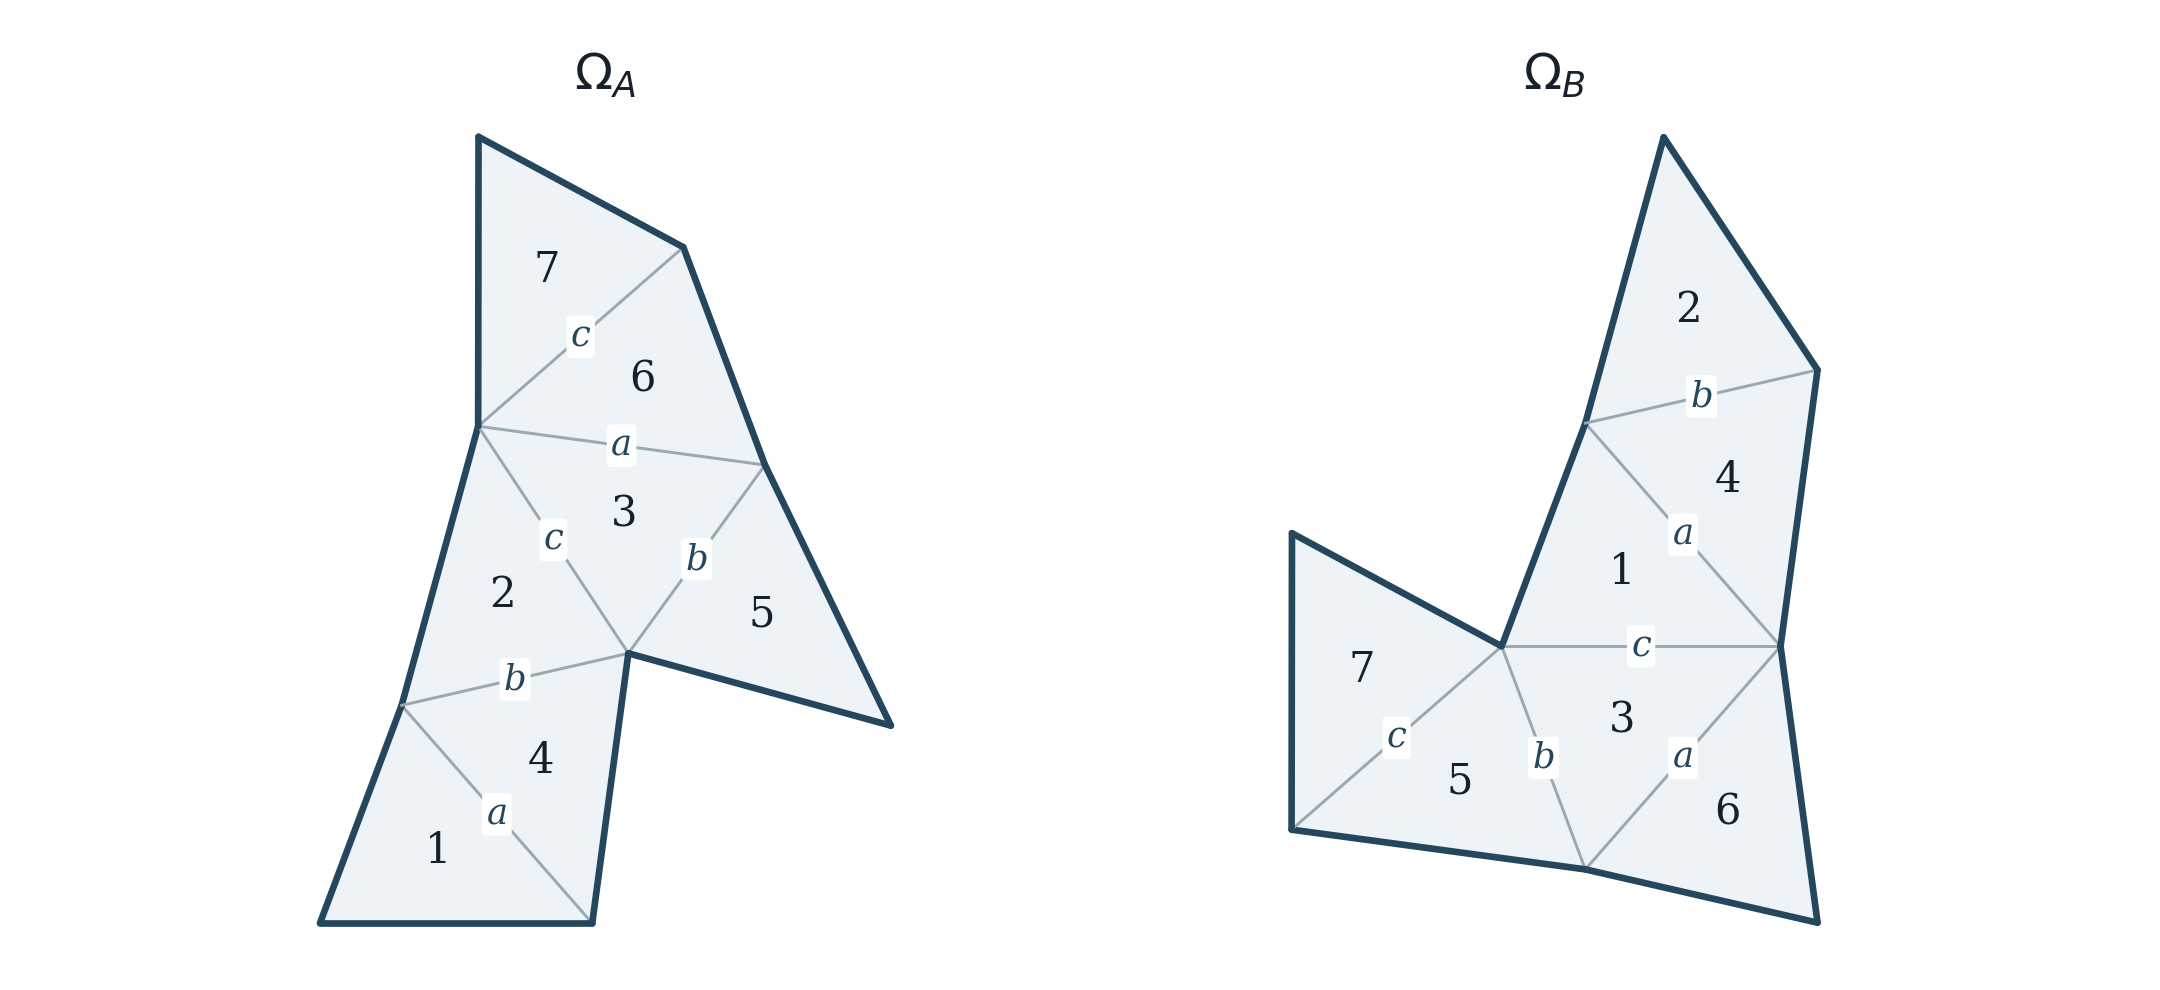
\includegraphics[width=0.73\linewidth]{figures/torsion-twins-paper.png}
\caption{Numbered tiles and labelled seams. Only the pairings along side $c$ differ.}
\label{fig:polygons}
\end{figure}

For each tile pair the separating-axis test finds an edge normal along
which one rational projection interval ends at or before the other
begins. Exact edge tests allow only common endpoints and prescribed
full seams. Each exposed vertex has degree two, and a walk visits all
nine exposed edges before returning to its start. The intersection tests
ensure that these edges meet only at consecutive endpoints. The simple
boundary and the connected gluing tree give simple connectivity.

\section{Transplantation}\label{sec:transplantation}

For each side $x$ and each polygon, define a symmetric signed permutation
matrix $X_x$. A glued pair $i,j$ contributes a $1$ in positions
$(i,j)$ and $(j,i)$. A fixed copy $i$ contributes $-1$ in position
$(i,i)$ for the Dirichlet condition and $+1$ for the Neumann condition.
All other entries are zero. In the Dirichlet case, the matrix
\[
 D=\begin{pmatrix}
 0& 1&0&-1&0&1&0\\
 1& 0&0&-1&1&0&0\\
 0& 0&1& 1&0&0&1\\
-1&-1&1& 0&0&0&0\\
 0& 1&0& 0&1&0&-1\\
 1& 0&0& 0&0&1&-1\\
 0& 0&1& 0&-1&-1&0
 \end{pmatrix}
\]
satisfies $D X_x^B=X_x^A D$ for $x=a,b,c$. For the Neumann case use
$N=(|D_{ij}|)$. Both determinants are $-24$. These are integer
identities checked directly by the verifier.

The transplantation argument can be written in terms of the energy
form \cite[Sections~3 and~6]{aek}.
Pull functions on the copies back to $T$. The Laplacian's form domain
then consists of $f\in H^1(T)^7$ with traces $X_x f=f$ on each side $x$.
This imposes matching traces across a seam and a zero trace at a
Dirichlet boundary side. For Neumann sides the trace is free. If $M$ is
$D$ or $N$, the matrix identity sends the form domain on $\twinB$ into
the one on $\twinA$. By symmetry of the signed permutations,
$M^{\mathsf T}$ maps the form domains in the reverse direction. With
$\mathcal E$ denoting the Dirichlet energy form, one has
\[
 \mathcal E_A(M f,h)=\mathcal E_B(f,M^{\mathsf T}h),\qquad
 \langle M f,h\rangle_A=\langle f,M^{\mathsf T}h\rangle_B .
\]
Both identities follow by summing over the isometric copies, with
$M$ constant on the tile. For each $\lambda$, $M$ maps the weak
$\lambda$-eigenspace on $\twinB$ into that on $\twinA$, and
$M^{\mathsf T}$ maps in the other direction. Since $\det M=-24$,
both maps are injective and the eigenspace dimensions agree.

\section{A certificate for the torsion gap}\label{sec:certificate}

\begin{lemma}\label{lem:variational}
For a bounded polygon $\Omega$, let $u\in H^1_0(\Omega)$ and let
$\sigma\in L^2(\Omega;\mathbb R^2)$ satisfy
$\operatorname{div}\sigma=-1$ in distributions. Then
\begin{equation}\label{eq:bounds}
 2\int_\Omega u\,\dd x-\int_\Omega|\nabla u|^2\,\dd x
 \ \le\ \tau(\Omega)\ \le\ \int_\Omega|\sigma|^2\,\dd x .
\end{equation}
\end{lemma}

\begin{proof}
Let $v$ be the weak solution of $-\Delta v=1$ with zero trace.
Testing with $v$ gives $\|\nabla v\|_2^2=\int_\Omega v=\tau(\Omega)$.
Testing with $u$ gives $\int_\Omega\nabla v\cdot\nabla u=\int_\Omega u$.
The squared norm $\|\nabla v-\nabla u\|_2^2$ gives the lower bound.
By density of $C_c^\infty(\Omega)$ in $H^1_0(\Omega)$, the distributional
divergence identity gives $\int_\Omega \sigma\cdot\nabla v=\int_\Omega v$.
It follows that
$\|\sigma\|_2^2-\tau(\Omega)=\|\sigma-\nabla v\|_2^2\ge0$.
\end{proof}

Subdivide each tile into $k^2$ triangles on the barycentric grid of step
$1/k$. The grids match along every glued side. For piecewise affine
$u$ and $\psi$, shared nodal values make their traces agree on every
mesh edge, including the seams. Both belong to $H^1(\Omega)$. Setting
$u=0$ at the boundary nodes gives $u\in H^1_0(\Omega)$. For the flux put
\[
 x_0=(1/2,1/2),\qquad
 \sigma(x)=-\tfrac12(x-x_0)+(\partial_2\psi,-\partial_1\psi).
\]
For any $\varphi\in C_c^\infty(\Omega)$, integration by parts gives
\[
 \int_\Omega(\partial_2\psi\,\partial_1\varphi-\partial_1\psi\,\partial_2\varphi)\,\dd x
 =-\int_\Omega\psi(\partial_2\partial_1\varphi-\partial_1\partial_2\varphi)\,\dd x=0.
\]
The rotated gradient has zero distributional divergence, so
$\operatorname{div}\sigma=-1$.

I used floating-point optimization to find the nodal values for $u$
and $\psi$, then rounded them to multiples of $2^{-50}$. The certificate
stores the integer numerators. The verifier requires one integer per
mesh node in each vector and checks that $u$ vanishes at each boundary
node. These conditions give admissible fields in \eqref{eq:bounds}.

On a small triangle
$K$ with area $A_K$, centroid $m_K$ and edge lengths $\ell_1,\ell_2,\ell_3$,
the verifier integrates $u$ as $A_K$ times its mean nodal value and
integrates $|\nabla u|^2$ as $A_K$ times the squared constant gradient.
Writing $w=(\partial_2\psi,-\partial_1\psi)|_K$, it uses
\[
 \int_K|\sigma|^2\,\dd x
   = A_K\left|w-\tfrac12(m_K-x_0)\right|^2
     +\frac{A_K}{144}(\ell_1^2+\ell_2^2+\ell_3^2).
\]
This follows from the centroid identity
$\int_K|x-m_K|^2\,\dd x=A_K\sum_i\ell_i^2/36$. Every quantity in the
integration uses rational coordinates or squared lengths.

The ancillary files include \texttt{torsion-witness-k64.json.gz} and
the verifier. From their directory run
\mbox{\texttt{python verify\_torsion\_twins.py 64}}. The verifier uses
only integer and rational arithmetic. For Table~\ref{tab:bounds} it
rounds the exact lower bounds down and the upper bounds up to nine
decimal places. Each mesh has $28\,672$ triangles. On Windows~11 with
CPython~3.14, the standard-library run took about $13$ seconds and
peaked at $50$ MiB.

\begin{table}[htb]
\centering
\begin{tabular}{@{}lrr@{}}
\toprule
Polygon & Lower bound & Upper bound\\
\midrule
$\twinA$ & $0.152472053$ & $0.152748988$\\
$\twinB$ & $0.152884186$ & $0.153162566$\\
\bottomrule
\end{tabular}
\caption{Certified enclosures of Dirichlet torsional rigidity at $k=64$.}
\label{tab:bounds}
\end{table}

The intervals in Table~\ref{tab:bounds} give a gap of at least
$0.000135198$. Rigid motions preserve torsional rigidity, so the
polygons are noncongruent. Equation~\eqref{eq:heat-torsion} now gives
different heat contents.

\section{The short-time expansion}\label{sec:short-time}

Each polygon has area $14/5$ and three exposed sides of each length.
They also have the same multiset of interior angles. To see this,
fix a vertex $v_x$ of $T$ and use the two columns of
Table~\ref{tab:gluing} for the sides incident to $v_x$. At each
corner the incident tiles form a single fan. A path component of
size $m$ therefore gives one corner of angle $m\theta_x$, where
$\theta_x$ is the angle of $T$ at $v_x$.
For $x=a,b$ the component sizes are $1,2,4$ in both polygons. For
$x=c$ they are $1,3,3$.

The polygonal heat-content formula of van den Berg and
Srisatkunarajah \cite[Theorem~1]{bs} gives the area term, a
$\sqrt t$ term determined by perimeter, and a $t$ term given by a
sum over the angles. The remainder is $O(e^{-c/t})$ for some $c>0$.
All three terms cancel in the difference, which completes
Theorem~\ref{thm:main}. The heat contents are analytic for $t>0$ by
their absolutely summable spectral weights. Since they differ, they
must differ at some time in every interval $(0,\varepsilon)$.

\newpage
\section{The role of the boundary condition}\label{sec:mirrors}

Gilkey's covering theorem gives $Q_{M_1}=kQ_{M_2}$ for a finite
$k$-sheeted Riemannian cover $M_1\to M_2$ of compact manifolds with
smooth boundary \cite[Theorem~2.2 and Section~2.5]{gilkey}. The proof pulls
back Dirichlet eigenfunctions, retaining the boundary condition and
pulling back the constant function to the constant function.
At an exposed mirror edge the Dirichlet heat solution extends oddly.
On the doubled tile, its initial datum is $+1$ on the original half
and $-1$ on the reflected half. Gilkey's argument uses the constant
initial datum on the covering space. That datum is even under
reflection, and the corresponding heat solution satisfies a Neumann
condition at the mirror. Theorem~\ref{thm:main} gives a pair for which
the all-Dirichlet heat contents differ.

The even choice has a direct consequence. Solve the heat equation
on one tile with Neumann conditions on the marked sides and
Dirichlet conditions on any unmarked boundary. Start at temperature
one. Place the solution on each copy. The traces match and the
normal flux vanishes on both sides of every seam, so the assembled
function solves the mixed heat equation. Its heat content is the
number of copies times that of the tile, regardless of the gluing.
For the triangles here, all sides are marked and the even problem
is pure Neumann. Its heat content is constant.

\paragraph{Disclosure.} The assistance of generative artificial intelligence was used in the development and implementation of code, though not in the formulation of the ideas behind the code.

\begin{thebibliography}{99}
\small
\raggedright
\bibitem{kac}
M. Kac, Can one hear the shape of a drum?,
\emph{Amer. Math. Monthly} \textbf{73} (1966), no.~4, part~II,
1--23. \doi{10.1080/00029890.1966.11970915}.

\bibitem{gww}
C. Gordon, D. Webb and S. Wolpert, Isospectral plane domains and
surfaces via Riemannian orbifolds, \emph{Invent. Math.}
\textbf{110} (1992), 1--22. \doi{10.1007/BF01231320}.

\bibitem{bcds}
P. Buser, J. Conway, P. Doyle and K.-D. Semmler, Some planar
isospectral domains, \emph{Int. Math. Res. Not.} (1994), no.~9,
391--400. \doi{10.1155/S1073792894000437}.

\bibitem{cm}
J. Comer and P. McDonald, Torsional rigidity and isospectral planar
sets, preprint (2021). \href{https://arxiv.org/abs/2105.07477}{arXiv:2105.07477}.

\bibitem{bdk}
M. van den Berg, E. B. Dryden and T. Kappeler, Isospectrality and heat
content, \emph{Bull. Lond. Math. Soc.} \textbf{46} (2014), 793--808.
\doi{10.1112/blms/bdu035}.

\bibitem{mm}
P. McDonald and R. Meyers, Isospectral polygons, planar graphs and heat
content, \emph{Proc. Amer. Math. Soc.} \textbf{131} (2003), 3589--3599.
\doi{10.1090/S0002-9939-03-07123-5}.

\bibitem{ckm}
D. Colladay, L. Kaganovskiy and P. McDonald, Torsional rigidity,
isospectrality and quantum graphs, \emph{J. Phys. A Math. Theor.}
\textbf{50} (2017), 035201. \doi{10.1088/1751-8121/50/3/035201}.

\bibitem{aek}
W. Arendt, A. F. M. ter Elst and J. B. Kennedy, Analytical aspects
of isospectral drums, \emph{Oper. Matrices} \textbf{8} (2014),
255--277. \doi{10.7153/oam-08-14}.

\bibitem{bs}
M. van den Berg and S. Srisatkunarajah, Heat flow and Brownian motion
for a region in $\mathbb R^2$ with a polygonal boundary,
\emph{Probab. Theory Related Fields} \textbf{86} (1990), 41--52.
\doi{10.1007/BF01207512}.

\bibitem{gilkey}
P. Gilkey, Heat content, heat trace, and isospectrality, in
\emph{New Developments in Lie Theory and Geometry},
Contemp. Math. \textbf{491}, Amer. Math. Soc., 2009, 115--123.
\href{https://arxiv.org/abs/0802.2948}{arXiv:0802.2948}.
\end{thebibliography}
\end{document}
